% LaTeX template for ECE 486 Lab; this template should be used with "report"
% section in the lab manual

% by Y\"un Han
% 2017-06-06

% A lot of changes have happened during the last four years. So a major overhaul
% is needed.

% -------------------
% Editor + TeX engine
% -------------------
% There are many online TeX services which require no local installation of TeX
% on your computer. Over the years, I have seen students use
% https://www.overleaf.com https://www.sharelatex.com among others although I
% have no direct experience of any of them. If you do not want any hassle of
% having a copy of TeX on your machine, or you don't mind privacy policies of
% those online services, you can use the online TeX system as well. They will
% serve you well, at least for our lab report.

% If you are really interested in beautiful print, and efficient editing, you
% can explore other options. For example, I use local TeX installations on my
% Linux, Mac and Windows machines. See the original preamble regarding how to
% choose a proper distribution for different platforms.

% As for editors, I use emacs + AUCTeX. You can enable major modes to handle
% *.tex files and minor modes to streamline your typesetting. For example, most
% people will use PDF mode rather than output files in *.ps or *.dvi these
% days; LaTeX-math-mode will speed up entering common math symbols and Greek
% letters; auto-complete will do a similar thing; flyspell mode will give you
% spell check etc.

% As for setting up emacs itself, you can check out Jess Hamrick's github repo
% https://github.com/jhamrick/emacs. I only enabled auctex, auto-complete,
% color-them-solarized, helm, helm-descbinds, and nyan-mode. To get these these
% packages installed, you can use el-get package management for emacs. 

% For ECE 486 however, portable set-up is already available on lab computers
% N:\labs\ECE486\ece486_Emacs_LaTeX
% Configuration files are also available from this repo
% https://github.com/yunlhan/ece486lab_latex/tree/master/emacs_latex

% ------------
% LaTeX how-to 
% ------------
% I use the following
% https://en.wikibooks.org/wiki/LaTeX
% https://en.wikibooks.org/wiki/LaTeX/Tips_and_Tricks
% https://tex.stackexchange.com

% ---------------
% Working example
% ---------------
% I wrote a book (127 pages) based on my lectures notes. You can scan the book
% and you may find it helpful when you use LaTeX. For example, how to handle
% cases in equations, how to selectively label questions, advanced graphics,
% references, just name a few. The book is in available in another repo
% https://github.com/yunlhan/ENT40days

% -------------
% Writing guide
% -------------
% You may find the Guardian style guide useful,
% https://www.theguardian.com/guardian-observer-style-guide-a Especially, their
% guide on "quotation marks" and "commas".

% -----------------------------------------------------------------------------

% original preamble
%
% This is the alpha version of lab report template in LaTeX. Inspired by the
% effort of Daniel Whisman (enrolled in ECE 486, Fall 2013)
% written by Y\"un L. Han.
% 2014-09-12

% It is recommended to use 
%
% TeXLive on Linux, url: http://tug.org/texlive/
% MacTex on Mac OS X, url: http://tug.org/mactex/
% MikTeX on Windows, url: http://miktex.org/

% For more info about how to use LaTeX (not TeX, TeX is a programming
% language, however LaTeX is not), see a quick guide from ECE Thesis wiki,

% https://wiki.cites.illinois.edu/wiki/display/ECEThesisReview/LaTeX+Resources

% Read the Documentation file ECE LaTeX Guide.pdf down at the bottom 
% of the page. As a starter, you only have to learn briefly how to typeset 
% equations and insert figures and other graphics. As an experienced user,
% however, you can grab the template and write your report immediately.

\documentclass{article}
\usepackage{graphicx}
\usepackage{caption}
\usepackage{mathtools} % load AMS maths
\usepackage{amsmath}  % for math spacing
\usepackage{amssymb}  % for math spacing
\usepackage{colortbl} % colour for table
\usepackage{xcolor} % define colours
\usepackage[margin=1in]{geometry} % an easy way to change page layout, Thanks to Brady Salz 
\usepackage{multirow}
\definecolor{Grey}{gray}{0.85}
% \setallmath{\displaymath}
\newcommand{\score}{\hfill \underline{\hspace{0.65cm}}\,/} % for score underline
\newcommand\RR{\textsuperscript{\textregistered}~} % for registered mark

\usepackage{listings}
\lstset{                  %设置代码块
    basicstyle=\small\ttfamily,% 基本风格
    numbers=left,    % 行号
    numbersep=10pt,  % 行号间隔
    tabsize=4,       % 缩进
    extendedchars=true, % 扩展符号?
    breaklines=true, % 自动换行
    frame=shadowbox,  % 框架左边竖线
    xleftmargin=19pt,% 竖线左边间距
    showspaces=false,% 空格字符加下划线
    showstringspaces=false,% 字符串中的空格加下划线
    showtabs=false,  % 字符串中的tab加下划线
    % keywordstyle=\bfseries\color{NavyBlue}, % 设置关键字为粗体,颜色为 NavyBlue
}

\begin{document}
% consider aligning your names like the following
% ----
% ************Lab X Report 
%
% ************by YOUR NAME
% ******Lab Partner: HIS/HER NAME
% ******Lab      TA: Y\"un Han
% ----
\title{\bf Lab \#2 Report\\{\sc Digital Simulation}}
\author{Tiantian Zhong\\ 3200110643 \\ Section LA1}
\maketitle
\noindent \fbox{\bf \Large Total: \underline{\hspace{0.65cm}}\,/50}
\section*{\sc Prelab Exercises}

We have
\[H(s)=\frac{Y(s)}{U(s)} = \frac{25}{s^2+6s+25} = \frac{25}{(s+3)^2 + 16}.\]

Thus
\[s^2 + 2\zeta \omega_n s + \omega_n^2 = s^2+6s+25\]

and we yields
\begin{align*}
\begin{cases}
              \zeta = \frac{3}{5} = 0.6 \\
              \omega_n = 5.  
\end{cases}
\end{align*}

Solve $s^2 + 6s + 25=0$ we have the poles 
\[s_{\text{poles}}=\frac{-6\pm \sqrt{36-100}}{2} = -3\pm 4j.\]

Figure \refeq{fig-prelab-diagram} shows the block diagram for this system.

% End of Prelab Exercises

\section{{\sc State Space Model of} $H_1(s)$\score 8}
(Compare the plots of \verb|y_dot| and \verb|y| obtained in Part 1 of the lab with the plots previously made for the prelab. Why are they identical? Attach plots---if your prelab plot was wrong, fix it and attach the corrected plot.)
% add your discussion here

The plots for Prelab and Part 1 are identicle. It is because the transfer function $H(s)$ in prelab can be written in state-space form:

% the following are templates for two FIGURES
\noindent The plots of $y$ and $\dot{y}$ from the prelab and lab are shown in Figures~\ref{fig:prelab2} and~\ref{fig:lab2-part1}.

% uncomment the following to insert your OWN figures
% \begin{figure}[htbp]
% \centering
% \includegraphics[width=0.88\linewidth]{prelab/prelab2_step.png}
% \caption{Plots of $y$ and $\dot{y}$, from the prelab, for a step input.}
% \label{fig:prelab2}
% \end{figure}

% \begin{figure}[htbp]
% \centering
% \includegraphics[width=0.88\linewidth]{lab2_step.png}
% \caption{Plots of $y$ and $\dot{y}$, from the lab, for a step input.}
% \label{fig:lab2}
% \end{figure}

\section{{\sc Effects of an extra Zero}\score 22}
% attach the figure in lab 2 of step responses after adding a zero
The step responses after adding an extra zero are shown in Figure~\ref{fig:effect_zeros}.
% \begin{figure}[htbp]
% \centering
% \includegraphics[width=0.84\linewidth]{zero_added.png}
% \caption{Effects of an extra zero on the step response.}
% \label{fig:effect_zeros}
% \end{figure}


\subsection{Effects of a Zero on $M_p$, $t_r$, and $t_s$\score 2}
Fill the table of specs of time domain responses.
% also attach a sample figure showing how you calculate the specs of the step responses [using your lab 0 script]

\begin{table}[phtb]\footnotesize 
\begin{center}
\caption{Effects of Zero}
\label{tbl:lab2_q2}
\begin{tabular}{c|c|c|c|c|c|c} \hline \hline
\rowcolor{Grey} & No zero & $H_2(s)$ zero &  $H_2(s)$ zero &  $H_2(s)$ zero  &  $H_2(s)$ zero &  $H_2(s)$ zero \\
\rowcolor{Grey} Specs & $H_1(s)$ & at $s = -30$ & at $s = -3$ &  at $s = -1.5$ &   at $s = 1.8$ &   at $s = 18$ \\ \hline
$M_p$\,[\%] &  & 10 &  &  &  &  \\ \hline
$t_r$\,[s] &  & 0.6 &  &  &  &  \\ \hline
$t_s$\,[s] &  & 0.4 &  &  &  & \\ \hline
\end{tabular}
\end{center}
\end{table}

\subsection{Discuss the Effects of a LHP Zero\score 4}
(Explain how $M_p$ , $t_r$ , and $t_s$ are affected by the zero location. When can the zero be ignored?)
% add your discussion here

\subsection{Effects of a Non-minimum Phase Zero\score 2}
(What is unique in this situation?)
% add your discussion here

\subsection{Decomposition of $H_2(s)$\score 14}
(Take $H_2(s)$, set $\zeta$ to the value found in the prelab, separate the numerator into two terms so that $H_2(s)$ is a sum of 2 fractions. Discuss how this decomposition helps to explain the effect of the zero location. In particular, discuss what each term represents. Also discuss $\alpha$'s effect. Which term dominates as $\alpha$ approaches 0? As $\alpha$approaches $\infty$?  What happens when $\alpha$ is negative?)

\begin{align*}
H_2(s) &=\frac{25 \left( 1+\frac{s}{\alpha \zeta} \right)}{s^2+10\zeta s +25}\\
       &= \mbox{\sc insert fraction 1} + \mbox{\sc insert fraction 2}
\end{align*}
% complete the above decomposition and add your discussion here

\section{{\sc Effects of an extra Pole}\score 20}
% attach the figure in lab 2 of step responses after adding a pole
The step responses after adding an extra pole are shown in Figure~\ref{fig:effect_pole}.
% uncomment the following to insert your OWN figure
% \begin{figure}[htbp]
% \centering
% \includegraphics[width=0.88\linewidth]{pole_added.png}
% \caption{Effects of an extra pole on the step response.}
% \label{fig:effect_poles}
% \end{figure}

\subsection{Effects of a Pole on $M_p$, $t_r$, and $t_s$\score 2}
(Fill out the table of specs of time domain responses.)
\begin{table}[phtb]
\begin{center}
\caption{Effects of Pole}
 \label{tbl:lab2_q3}
\begin{tabular}{c|c|c|c|c} \hline \hline
\rowcolor{Grey} & No pole & $H_2(s)$ pole & $H_2(s)$ pole & $H_2(s)$ pole \\
\rowcolor{Grey} Specs &  $H_1(s)$ &  at $s = -30$ &  at $s = -3$ & at $s = -1.5$ \\ \hline   
$M_p$\,[\%] &  &  &  &  \\ \hline
$t_r$\,[s] &  &  &  &  \\ \hline
$t_s$\,[s] &  &  &  &  \\ \hline
\end{tabular}
\end{center}
\end{table}

\subsection{Discuss the Effects of an Extra Pole\score 4}
(Explain how $M_p$ , $t_r$ , and $t_s$ are affected by the location of the additional pole. When can the extra pole be ignored?)
% add your discussion here

\subsection{Decomposition of $H_3(s)$\score 14}
\begin{align*}
H_3(s) &= \frac{25}{\left(1+\frac{s}{\alpha \zeta}\right)\left( s^2 + 10 \zeta s + 25\right) } \mbox{~~~($\zeta = 0.6$)} \\
&= \frac{k_1}{1+\frac{5s}{3\alpha}} + \frac{k_2 s}{s^2+6s+25} + \frac{k_3}{s^2+6s+25}
\end{align*}
Using a partial fraction expansion,
\begin{align*}
k_1 &= -\frac{25}{\alpha^2 \zeta^2 - 10 \alpha\zeta + 25}\\
k_2 &= -\frac{25\alpha\zeta}{\alpha^2 \zeta^2 -10\alpha\zeta + 25}\\
k_3 &= 25+\frac{625}{\alpha^2 \zeta^2 - 10\alpha\zeta + 25}
\end{align*}
(Discuss how this decomposition helps to explain the effect of the location of an additional pole. In particular, discuss what each term represents. Also discuss $\alpha$'s effect. Which term dominates as $\alpha$ approaches 0? As $\alpha$ approaches $\infty$?)
% add your discussions about the above decomposition
\newline \\[10mm]
\noindent {\bf \large Attachments}
\begin{itemize}
\item Plot from the prelab
\item Plots of overlaid step responses after adding a zero; and after adding a pole
\item Sample figures for calculating $M_p$ , $t_s$ and $t_r$ in Table~\ref{tbl:lab2_q2} and Table~\ref{tbl:lab2_q3}
\item {\sc Matlab} code
\end{itemize}

\pagebreak
\section*{Attachments}
\subsection*{Plots}
\begin{figure}[h!]
       \centering
       \includegraphics[width=0.8\textwidth]{figs/prelab_blocks.png}
       \caption{Block diagram of $H(s) = \frac{25}{s^2+6s+25}$}
       \label{fig-prelab-diagram}
\end{figure}

\begin{figure}[h!]
       \centering
       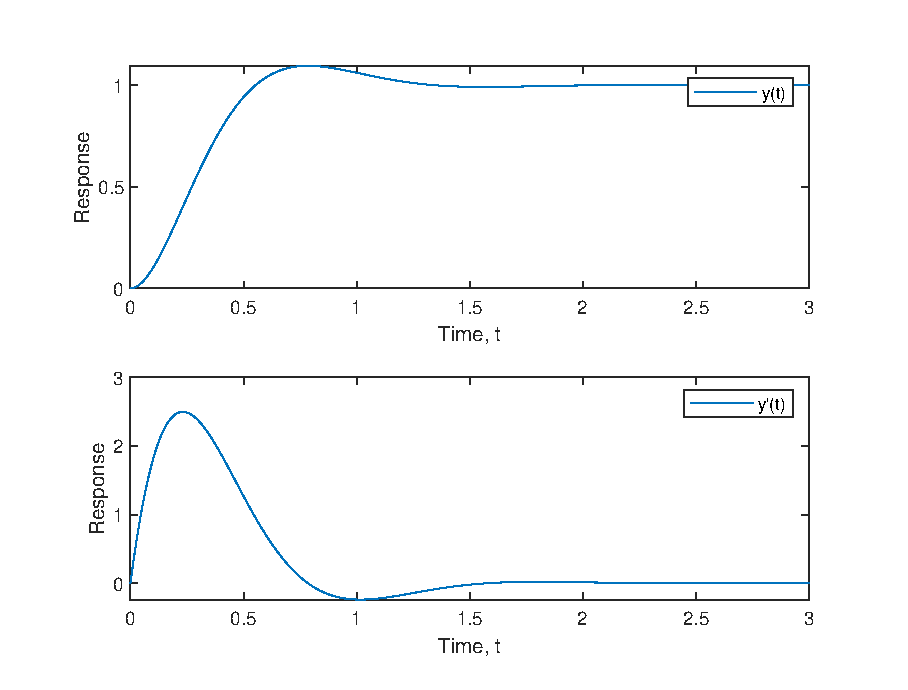
\includegraphics[width=0.7\textwidth]{figs/prelab_plot.eps}
       \caption{Plot from the prelab}
       \label{fig:prelab2}
\end{figure}

\begin{figure}[h!]
       \centering
       \includegraphics[width=0.7\textwidth]{figs/part_1_plot.eps}
       \caption{Plot from part 1}
       \label{fig:lab2-part1}
\end{figure}

\newpage
\subsection*{\textsc{Matlab} Code}


\end{document}